\section{Experimental Results}
\label{sec:experiments}

In this section, we present empirical evidence to verify our theoretical findings. We train ResNet \citep{He2016DeepResNet} and VGG \citep{Simonyan14VGG} on CIFAR10 \citep{Krizhevsky2009CIFAR}. To simulate data heterogeneity in CIFAR-10, we impose label imbalance across clients, i.e. each client is allocated a proportion of the samples of each label according to a Dirichlet distribution \citep{Hsu2019MeasuringTE, Yurochkin2019BayesianNF}. The concentration parameter $\alpha>0$ indicates the level of \textit{non-i.i.d.}, with smaller $\alpha$ implies higher heterogeneity, and $\alpha\to\infty$ implies \textit{i.i.d.} setting. Unless specified otherwise, we have 100 clients in all experiments, and the partial participation ratio is 0.05, i.e., 5 out of 100 clients are picked in each round, \textit{non-i.i.d.} is $\alpha=0.5$, and local epoch is 3. We defer many more results and details of hyperparameter settings to Appendix \ref{sec:appendix_exp}.

\subsection{Results on FedGM}
\label{subsec:exp_fedgm}

Figure \ref{fig:resnet_cifar10} shows the results for ResNet on CIFAR-10 with FedGM, FedAvgM, and FedAvg. We perform grid search over $\eta\in\{0.5,1.0,1.5,\dots,5.0\}$, $\beta\in\{0.7,0.9,0.95\}$, and $\nu\in\{0.7,0.9,0.95\}$. We report their respective best results in Figure \ref{fig:resnet_cifar10}. We observe that though FedAvgM converges faster than FedAvg, it is only marginally better in terms of testing. FedGM, in contrast, outperforms FedAvgM and FedAvg in both measures. Therefore, a general momentum, instead of only SHB, is critical empirically. We analyze possible reasons and leave more results with VGG and different heterogeneity levels $\alpha$ to Appendix \ref{subsec:appendix_more_results_fedgm}.

\iffalse

\begin{figure}[h]

\centering
\subfigure{
\hspace{0pt}
\includegraphics[width=.22\textwidth]{figs/resnet_cifar10_train.eps}
\label{subfig:resnet_cifar10_train}
}
\hspace{-6pt}
\subfigure{
\includegraphics[width=.22\textwidth]{figs/resnet_cifar10_test.eps}
\label{subfig:resnet_cifar10_test}
}

\caption{\ref{subfig:resnet_cifar10_train} Training and \ref{subfig:resnet_cifar10_test} Testing Curves for ResNet on CIFAR-10. FedGM outperforms FedAvg/FedAvgM.}
\label{fig:resnet_cifar10}
\vspace*{-10pt}
\end{figure}

\subsection{Results on Multistage FedGM}
\label{subsec:exp_multistage_fedgm}

\fi




\subsection{Results on Multistage FedGM}
\label{subsec:exp_multistage_fedgm}


Figure \ref{fig:resnet_cifar10_multistage} shows the results for ResNet on CIFAR-10 with multistage vs. single-stage FedGM. The two black vertical lines at round 143 and 429 mark the end of 1st/2nd stage. For multistage FedGM, $(\eta_1=2.0,\eta_2=1.0,\eta_3=0.5)$, the $\beta$ also changes according to Eq. \ref{stagewise_hyper_constraints}. From Figure \ref{fig:resnet_cifar10_multistage}, we observe multistage FedGM is better than single-stage FedGM, no matter what constant $\eta$ it takes. Specifically, at first stage, $\eta_1=2.0$ makes the training curve fluctuate dramatically, but later into 2nd/3rd stage, the training stabilizes with smaller $\eta_2$ and $\eta_3$. Multistage FedGM achieves a balance between early exploration and late exploitation. Multistage is also superior to its counterpart in testing. We leave more experiments to Appendix \ref{subsec:more_exp_multistage_appendix}.

\begin{figure}[h]

\centering
\subfigure{
\hspace{0pt}
\includegraphics[width=.35\textwidth]{figs/multistage_train.eps}
\label{subfig:multistage_resnet_cifar10_train}
}
\subfigure{
\hspace{0pt}
\includegraphics[width=.35\textwidth]{figs/multistage_test.eps}
\label{subfig:multistage_resnet_cifar10_test}
}

\caption{\ref{subfig:multistage_resnet_cifar10_train} Training and \ref{subfig:multistage_resnet_cifar10_test} Testing Curves for Multistage FedGM vs. Single-stage FedGM.}
\label{fig:resnet_cifar10_multistage}
\end{figure}




\subsection{Results on Autonomous FedGM}
\label{subsec:exp_autonomous_fedgm}

Figure \ref{fig:resnet_cifar10} shows the results for ResNet on CIFAR-10 with Autonomous FedGM (\& FedAvg). Please refer to Appendix \ref{subsec:exp_settings_appendix} for detailed settings. We perform a grid search as in Section \ref{subsec:exp_fedgm}. We report their respective best curves. We plot an ideal FedGM (i.e. synchronous and identical local epochs) as reference line. We could observe Autonomous FedGM outperforms Autonomous FedAvg with system heterogeneity. Though Autonomous FedGM suffers a slowdown compared to the ideal FedGM, it is within a small margin, which supports our theory in Corollary \ref{corollary:free_multistage_fedgm_rate} and validates the effectiveness of Autonomous FedGM. We leave more experiments to Appendix \ref{subsec:appendix_more_exp_autonomous}.






